% \section{Integrando el dataset Físico-Químico y el Genómico}

Finalmente, unimos los dos conjuntos de variables para evaluar si la integración de ambos datasets representan una mejora frente a los resultados del modelo Genómico y Físico-Químico por separado. A este nuevo dataset lo denominamos dataset Integral. Las variantes usadas fueron nuevamente las encontradas en la tabla Humsavar. 

\section{Creación del dataset Integral}

El dataset Integral posee 68,508 variantes (la misma cantidad de variantes del dataset Físico-Químico), con 64 variables, que son las variables sumadas de los datasets Genómico (14), Físico-Químico (49) y la variable de respuesta. Del total de las variantes, 39,653 (58\%) son benignas y 28,855 (42\%) son patogénicas. Con respecto a los nulos, mantenemos la misma cobertura de las variables físico-químicas del dataset homónimo (aproximadamente 35\% para las variables categóricas y una cobertura mayor del 60\% para las continuas), mientras que para las variables genómicas tenemos alrededor de un 20\% de variantes que no poseen cobertura al no tener un identificador rsID.

\section{Generación del modelo}

Para este modelo preliminar utilizamos nuevamente el algoritmo Random Forest, repitiendo las mismas fases de imputación y entrenamiento usadas previamente en los modelos Genómico y Físico-Químico. Es decir, que en la fase de imputación usamos la mediana para los valores nulos de las variables continuas y el valor más frecuente en las variables categóricas. El entrenamiento consistió en una búsqueda de hiperparámetros óptimos usando \textit{GridSearch} en un diccionario de posibles parámetros, evaluados en una triple validación cruzada basándonos en el AUC como métrica a optimizar. El dataset de entrenamiento posee 45,900 variantes, aproximadamente dos tercios del dataset completo. Una vez entrenado el modelo usando este \textit{pipeline}, se evaluaron las variantes del dataset de testeo, es decir, el tercio restante del dataset completo. Posteriormente utilizamos un método de boosting, Xtreme Gradient Boosting (XGBoost). Los hiperparámetros de este método fueron elegidos usando una búsqueda randomizada (Randomized Grid Search). Este método de optimización fue elegido dado que las combinaciones que se evalúan en el método Grid Search son demasiadas. La búsqueda randomizada evalúa las mismas alternativas pero eligiendo combinaciones de forma aleatoria, sin probar todas las combinaciones. También es posible evaluar valores tomados de acuerdo a una distribución específica.

\section{Resultados del modelo Integral}

El modelo Random Forest obtuvo un AUC de 0.88. Esto representa una mejora con respecto al modelo Genómico (0.85) y al modelo Físico-Químico (0.72). Si comparamos las métricas obtenidas en el modelo Genómico con las de este modelo (figura \ref{tab:metrics_integral_rf}), se puede apreciar un nuevo salto en el \textit{recall} de las variables patogénicas, que pasa de un 0.64 en el modelo Genómico al 0.80, lo que representa un 16\% de mejora. También mejora la precisión con respecto a la detección de esta clase, que pasa de 0.69 a 0.76. La única métrica que decae es el \textit{recall} de la clase Benigna, que pasa de 0.87 a 0.82, lo que representa una leve caída del \textit{f1-score}. El modelo XGBoost superó la performance de Random Forest alcanzando un AUC de 0.90.


\begin{table}[H]
\centering
\begin{tabular}{|l|l|l|l|l|l|l|}
\hline
Modelo & Precisión & Recall & AUC & F1-score & $t_{fit}$ & $t_{pred}$ \\ \hline
RF & 0.76 & 0.80 & 0.88 & 0.78 & 2m 2 s & 0.3 s \\ \hline
XGB & 0.78 & 0.82 & 0.90 & 0.80 & 12m 47s & 1.14 s \\ \hline
\end{tabular}
\label{tab:metrics_model}

\caption{Comparación de métricas de modelos usando el dataset Integral. Las variables $t_{fit}$ y $t_{pred}$ corresponden al tiempo de entrenamiento y de predicción de todas las variantes \todo{REFERENCIAR}.}
\end{table}


\begin{table}[H]
\centering
\begin{tabular}{|l|l|l|l|}
\hline
Clase        & Precisión & Recall & F1-score \\ \hline
Benignas     & 0.85      & 0.82   & 0.83     \\ \hline
Patogénicas  & 0.76      & 0.80   & 0.78     \\ \hline
Promedio     & 0.81      & 0.81   & 0.81     \\ \hline
\end{tabular}
\caption{Reporte de métricas del modelo Random Forest usando el dataset Integral.}
\label{tab:metrics_integral_rf}
\end{table}


\begin{table}[H]
\centering
\begin{tabular}{|l|l|l|l|}
\hline
Clase        & Precisión & Recall & F1-score \\ \hline
Benignas     & 0.86      & 0.83   & 0.84     \\ \hline
Patogénicas  & 0.78      & 0.82   & 0.80     \\ \hline
Promedio     & 0.83      & 0.82   & 0.82     \\ \hline
\end{tabular}
\caption{Reporte de métricas del modelo XGB usando el dataset Integral.}
\label{tab:metrics_integral_xgb}
\end{table}




\section{Importancia de las variables}

Pasamos a analizar las importancias descriptas en la figura \ref{fig:importances_integral}. Nuevamente encontramos en primer lugar a las variables de conservación genómicas, resultado esperable dado su nivel de importancia en el dataset Genómico y su nivel de AUC conseguido. También encontramos en un segundo escalón a las variables de conservación a nivel de exones, y a una variable que considera el número de SNPs en el exón donde ocurre la mutación. Luego encontramos al grupo de matrices de sustitución de aminoácidos (EX, GRANTHAM, BLOSUM y PAM250), que también aparecieron en los primeros lugares en el modelo Físico-Químico. Por último encontramos una variable relativa a la clase funcional a nivel genómico (MISSENSE) y otra relativa al cambio de polaridad del aminoácido donde ocurre la variante (POLARITY), por lo que encontramos en nuestro ranking una lista de variables transversal a los dos datasets usados. 

En la figura \ref{fig:importance_cluster_integral_rf} unimos las variables de alta correlación en clusters y evaluamos su impacto en la precisión del modelo es la matriz GRANTHAM.



% Dada la alta correlación entre algunas variables que observamos en los modelos anteriores, en esta ocasión 


\begin{figure}[H]
    \centering
    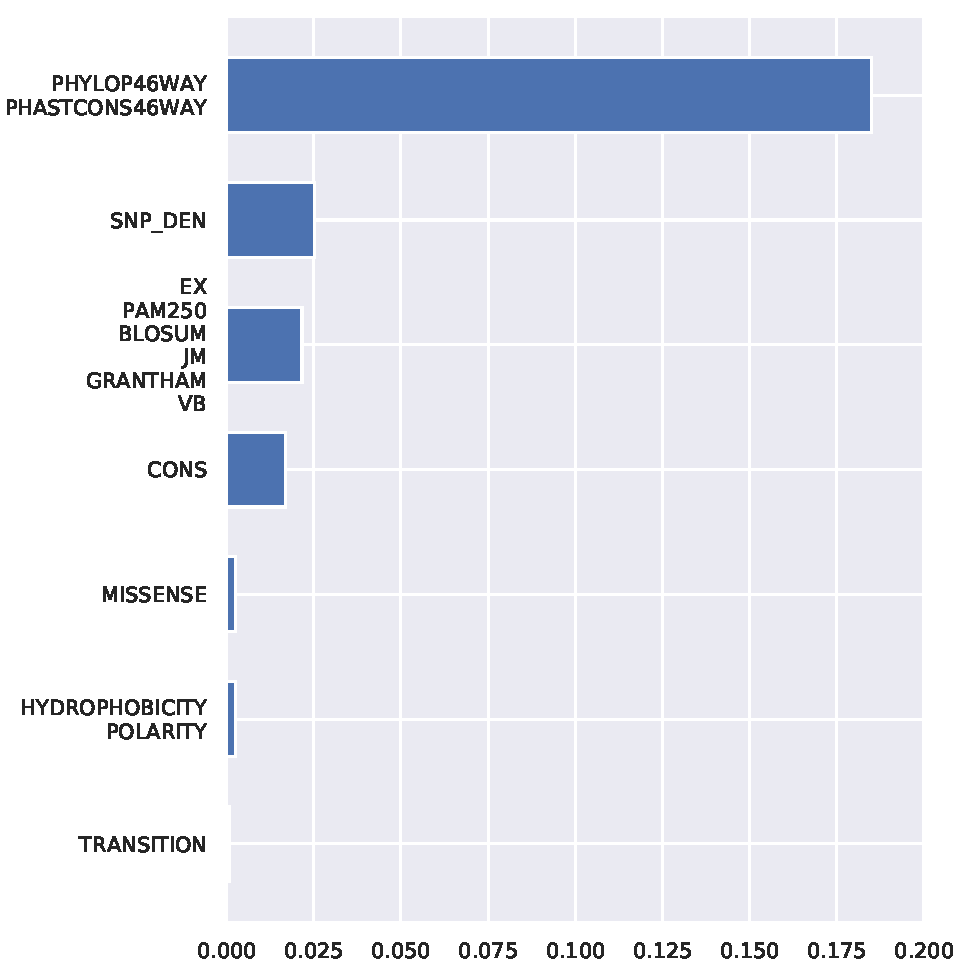
\includegraphics[scale=0.6]{documents/latex/figures/3/integral/integral_importance_cluster.pdf}
    \caption{Importancia de variables clusterizadas (basados en correlación de Spearman) usando permutación. Resultados del modelo usando Random Forest.}
    \label{fig:importance_cluster_integral_rf}
\end{figure}



\begin{figure}[H]
    \centering
    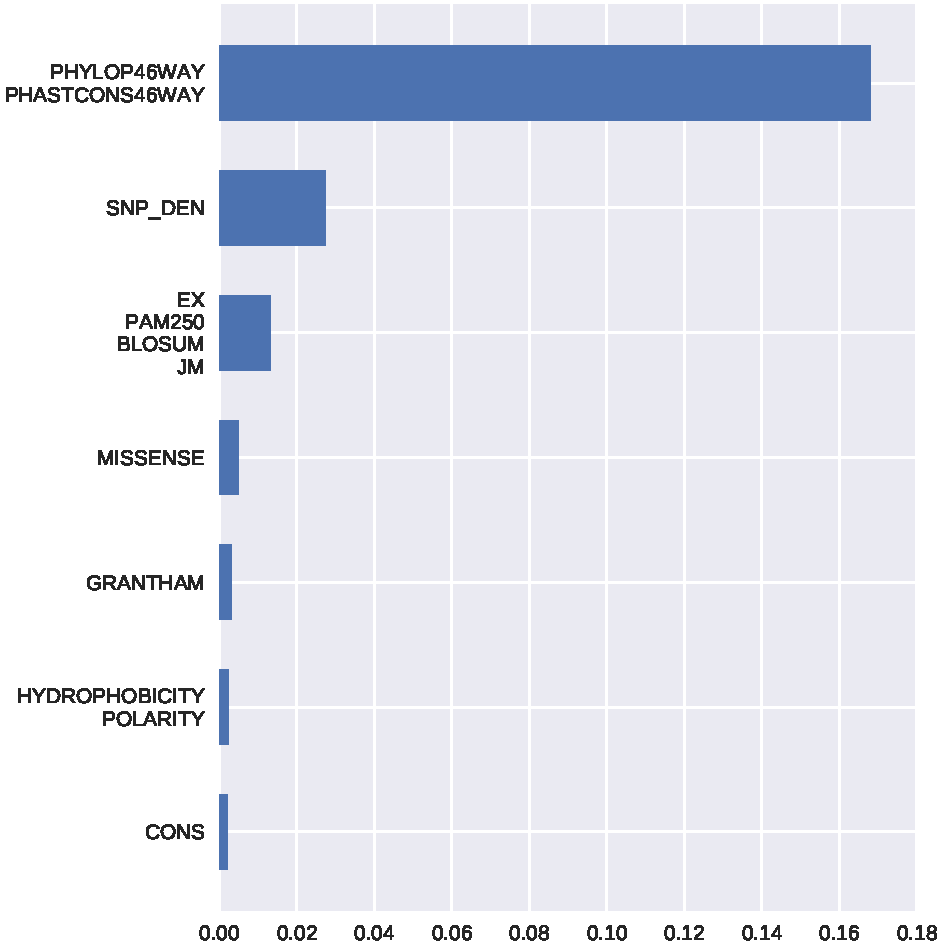
\includegraphics[scale=0.6]{documents/latex/figures/3/integral/integral_importance_cluster_xgb.pdf}
    \caption{Importancia de variables clusterizadas (basados en correlación de Spearman) usando permutación. Resultados del modelo usando XGB.}
    \label{fig:importance_cluster_integral_xgb}
\end{figure}


\newpage

\begin{figure}[H]
\centering
\begin{subfigure}[t]{0.7\textwidth}
    \centering
    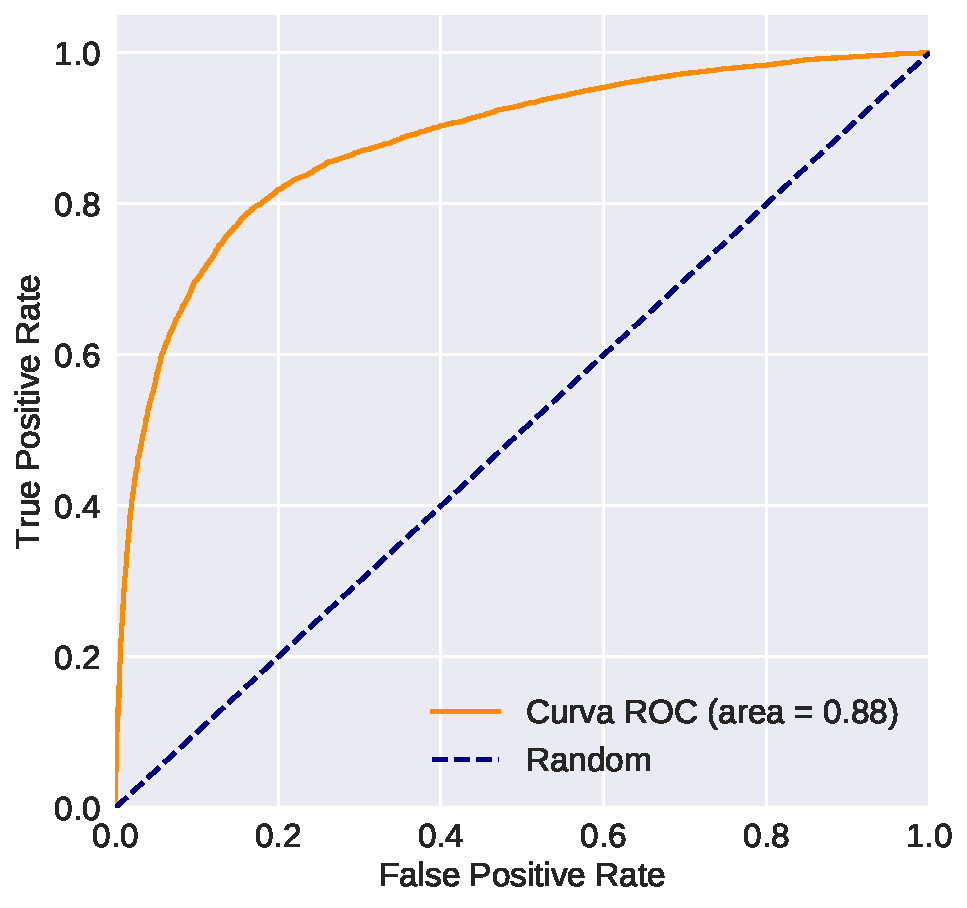
\includegraphics[width=\textwidth]{documents/latex/figures/3/integral/auc_integral.pdf}
    \caption{Comparación de curvas AUC entre algoritmos Random Forest y XGBoost. La línea punteada corresponde a un predictor Random.}
    \label{fig:auc_integral}
\end{subfigure}
\hfill
\hfill
\begin{subfigure}[b]{0.7\textwidth}
    \centering
    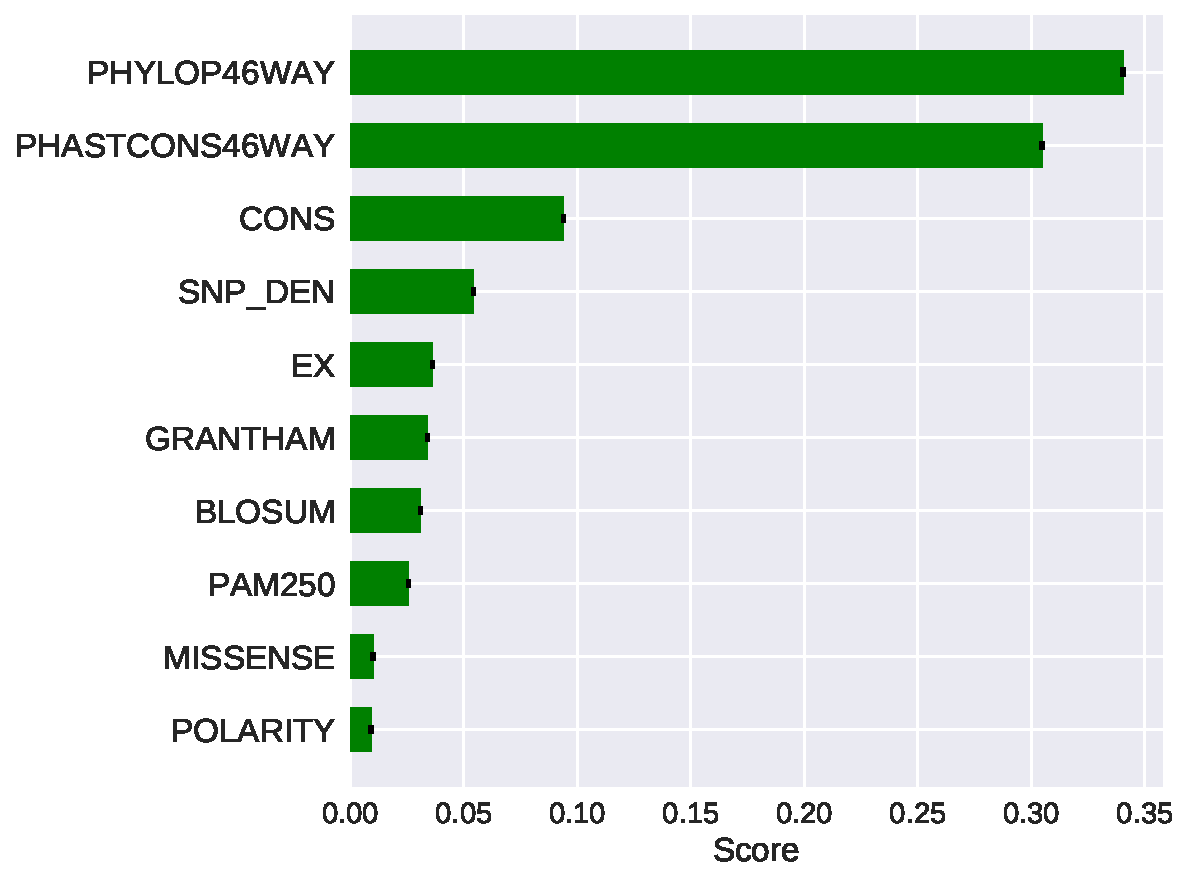
\includegraphics[width=\textwidth]{documents/latex/figures/3/integral/importances_integral.pdf}
    \caption{Los 10 atributos más importantes del dataset Integral aportados por el algoritmo Random Forest.}
    \label{fig:importances_integral}
\end{subfigure}

\caption{Curva AUC y atributos más importantes del modelo Integral.}

\end{figure}
